%{{第七十九回}}{第七十九回}}
\chapter{薛文龙悔娶河东狮\\贾迎春误嫁中山狼}

{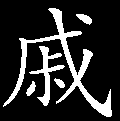
\includegraphics[width=3mm]{../Images/00005}\kaishu 静含天地自宽,动荡吉凶难定。一啄一饮系生成,何必梦中说醒。}

话说宝玉祭完了晴雯,只听花影中有人声,倒唬了一跳。及走出来细看,不是别人,却是林黛玉,满面含笑,口内说道:``好新奇的祭文!可与曹娥碑并传的了。''宝玉听了,不觉红了脸,笑答道:``我想着世上这些祭文都蹈于熟滥了,所以改个新样,原不过是我一时的顽意,谁知又被你听见了。有什么大使不得的,何不改削改削。''

黛玉道:``原稿在那里?倒要细细一读。长篇大论,不知说的是什么,只听见中间两句,什么`红绡帐里,公子多情,黄土垄中,女儿薄命。'这一联意思却好,只是`红绡帐里'未免熟滥些。放着现成真事,为什么不用?''宝玉忙问:``什么现成的真事?''黛玉笑道:``咱们如今都系霞影纱糊的窗槅,何不说`茜纱窗下,公子多情'呢?''宝玉听了,不禁跌足笑道:``好极,是极!到底是你想的出,说的出。可知天下古今现成的好景妙事尽多,只是愚人蠢子说不出想不出罢了。但只一件:虽然这一改新妙之极,但你居此则可,在我实不敢当。''说着,又接连说了一二百句``不敢''。

黛玉笑道:``何妨。我的窗即可为你之窗,何必分晰得如此生疏。古人异姓陌路,尚然同肥马,衣轻裘,敝之而无憾,何况咱们。''宝玉笑道:``论交之道,不在肥马轻裘,即黄金白璧,亦不当锱铢较量。倒是这唐突闺阁,万万使不得的。如今我越性将`公子'`女儿'改去,竟算是你诔他的倒妙。况且素日你又待他甚厚,故今宁可弃此一篇大文,万不可弃此`茜纱'新句。竟莫若改作`茜纱窗下,小姐多情,黄土垄中,丫鬟薄命。'如此一改,虽于我无涉,我也是惬怀的。''黛玉笑道:``他又不是我的丫头,何用作此语。况且小姐丫鬟亦不典雅,等我的紫鹃死了,我再如此说,还不算迟。''{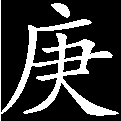
\includegraphics[width=3mm]{../Images/00004}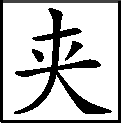
\includegraphics[width=3mm]{../Images/00012}\footnotesize \kaishu 明是为与阿颦作谶,却先偏说紫鹃,总用此狡猾之法。}宝玉听了,忙笑道:``这是何苦又咒他。''{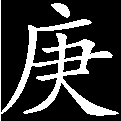
\includegraphics[width=3mm]{../Images/00004}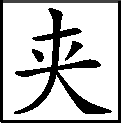
\includegraphics[width=3mm]{../Images/00012}\footnotesize \kaishu 又画出宝玉来,究竟不知是咒谁,使人一笑一叹。}黛玉笑道:``是你要咒的,并不是我说的。''宝玉道:``我又有了,这一改可妥当了。莫若说:`茜纱窗下,我本无缘;{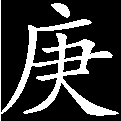
\includegraphics[width=3mm]{../Images/00004}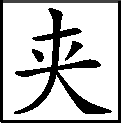
\includegraphics[width=3mm]{../Images/00012}\footnotesize \kaishu 双关句,意妥极。}黄土垄中,卿何薄命。'''{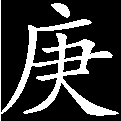
\includegraphics[width=3mm]{../Images/00004}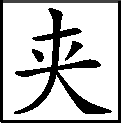
\includegraphics[width=3mm]{../Images/00012}\footnotesize \kaishu 如此我亦谓妥极。但试问当面用``尔''``我''字样,究竟不知是为谁之谶,一笑一叹。◇一篇诔文总因此二句而有,又当知虽诔晴雯而又实诔黛玉也。奇幻至此!若云必因晴雯诔,则呆之至矣。}

黛玉听了,忡然变色,{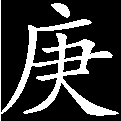
\includegraphics[width=3mm]{../Images/00004}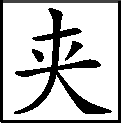
\includegraphics[width=3mm]{../Images/00012}\footnotesize \kaishu 慧心人可为一哭。观此句便知诔文实不为晴雯而作也。}心中虽有无限的狐疑乱拟,{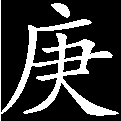
\includegraphics[width=3mm]{../Images/00004}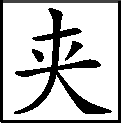
\includegraphics[width=3mm]{../Images/00012}\footnotesize \kaishu 用此事更妙,盖又欲瞒观者。}外面却不肯露出,反连忙含笑点头称妙,说:``果然改的好。再不必乱改了,快去干正经事罢。才刚太太打发人叫你明儿一早快过大舅母那边去。你二姐姐已有人家求准了,想是明儿那家人来拜允,所以叫你们过去呢。''宝玉拍手道:``何必如此忙?我身上也不大好,明儿还未必能去呢。''黛玉道:``又来了,我劝你把脾气改改罢。一年大二年小,\ldots{}\ldots{}''一面说话,一面咳嗽起来。{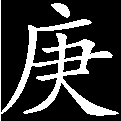
\includegraphics[width=3mm]{../Images/00004}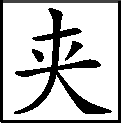
\includegraphics[width=3mm]{../Images/00012}\footnotesize \kaishu 总为后文伏线。阿颦之{(问)}{[}文{]}可见不是一笔两笔所写。}宝玉忙道:``这里风冷,咱们只顾呆站在这里,快回去罢。''黛玉道:``我也家去歇息了,明儿再见罢。''说着,便自取路去了。

宝玉只得闷闷的转步,又忽想起来黛玉无人随伴,忙命小丫头子跟了送回去。自己到了怡红院中,果有王夫人打发老嬷嬷来,吩咐他明日一早过贾赦那边去,与方才黛玉之言相对。

原来贾赦已将迎春许与孙家了。这孙家乃是大同府人氏,{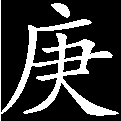
\includegraphics[width=3mm]{../Images/00004}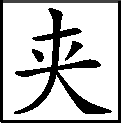
\includegraphics[width=3mm]{../Images/00012}\footnotesize \kaishu 设云``大概相同''也,若必云真大同府则呆。}祖上系军官出身,乃当日宁荣府中之门生,算来亦系世交。如今孙家只有一人在京,现袭指挥之职,此人名唤孙绍祖,生得相貌魁梧,体格健壮,弓马娴熟,应酬权变,{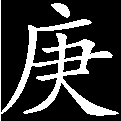
\includegraphics[width=3mm]{../Images/00004}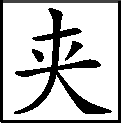
\includegraphics[width=3mm]{../Images/00012}\footnotesize \kaishu 画出一个俗物来。}年纪未满三十,且又家资饶富,{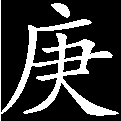
\includegraphics[width=3mm]{../Images/00004}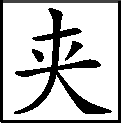
\includegraphics[width=3mm]{../Images/00012}\footnotesize \kaishu 此句断不可少。}现在兵部候缺题升。因未有室,贾赦见是世交子侄,且人品家当都相称合,遂青目择为东床娇婿。亦曾回明贾母。

贾母心中却不十分称意,想来拦阻亦恐不听,儿女之事自有天意前因,况且他是亲父主张,何必出头多事,为此只说``知道了''三字,馀不多及。贾政又深恶孙家,虽是世交,当年不过是彼祖希慕荣宁之势,有不能了结之事才拜在门下的,并非\elegantpar{诗礼名族之裔}{英美所谓old money},因此倒劝谏过两次,无奈贾赦不听,也只得罢了。

宝玉却从未会过这孙绍祖一面的,次日只得过去聊以塞责。只听见说娶亲的日子甚急,不过今年就要过门的,又见邢夫人等回了贾母将迎春接出大观园去等事,越发扫去了兴头,每日痴痴呆呆的,不知作何消遣。又听得说陪四个丫头过去,更又跌足自叹道:``从今后这世上又少了五个清洁人了。''因此天天到紫菱洲一带地方徘徊瞻顾,见其轩窗寂寞,屏帐翛然,不过有几个该班上夜的老妪。{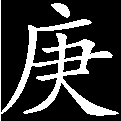
\includegraphics[width=3mm]{../Images/00004}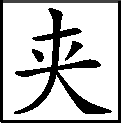
\includegraphics[width=3mm]{../Images/00012}\footnotesize \kaishu 先为``对{(竟)}{[}景{]}悼颦儿''作引。}再看那岸上的蓼花苇叶,池内的翠荇香菱,也都觉摇摇落落,似有追忆故人之态,迥非素常逞妍斗色之可比。既领略得如此寥落凄惨之景,是以情不自禁,乃信口吟成一歌曰:{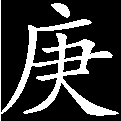
\includegraphics[width=3mm]{../Images/00004}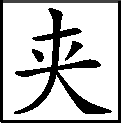
\includegraphics[width=3mm]{../Images/00012}\footnotesize \kaishu 此回题上半截是``悔娶河东狮'',今却偏逢``中山狼'',倒装上下情孽,细腻写来,可见迎春是书中正传,阿呆夫妻是副,宾主次序严肃之至。其婚娶俗礼一概不及,只用宝玉一人过去,正是书中之大旨。}

池塘一夜秋风冷,吹散芰荷红玉影。

蓼花菱叶不胜愁,重露繁霜压纤梗。

不闻永昼\elegantpar{敲棋}{妙}声,燕泥点点污棋枰。

古人惜别怜朋友,况我今当手足情!

宝玉方才吟罢,忽闻背后有人笑道:``你又发什么呆呢?''宝玉回头忙看是谁,原来是香菱。宝玉便转身笑问道:``我的姐姐,你这会子跑到这里来做什么?许多日子也不进来逛逛。''香菱拍手笑嘻嘻的说道:``我何曾不来。如今你哥哥回来了,那里比先时自由自在的了。才刚我们奶奶使人找你凤姐姐的,竟没找着,说往园子里来了。我听见了这信,我就讨了这件差进来找他。遇见他的丫头,说在稻香村呢。如今我往稻香村去,谁知又遇见了你。我且问你,袭人姐姐这几日可好?怎么忽然把个晴雯姐姐也没了,到底是什么病?二姑娘搬出去的好快,你瞧瞧这地方好空落落的。''

宝玉应之不迭,又让他同到怡红院去吃茶。{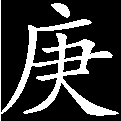
\includegraphics[width=3mm]{../Images/00004}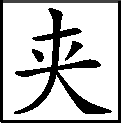
\includegraphics[width=3mm]{../Images/00012}\footnotesize \kaishu 断不可少。}香菱道:``此刻竟不能,等找着琏二奶奶,说完了正经事再来。''宝玉道:``什么正经事这么忙?''香菱道:``为你哥哥娶嫂子的事,所以要紧。''{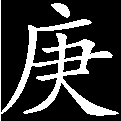
\includegraphics[width=3mm]{../Images/00004}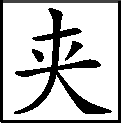
\includegraphics[width=3mm]{../Images/00012}\footnotesize \kaishu 出题,却闲闲引出。}宝玉道:``正是。说的到底是那一家的?只听见吵嚷了这半年,今儿又说张家的好,明儿又要李家的,后儿又议论王家的。这些人家的女儿他也不知道造了什么罪了,叫人家好端端议论。''香菱道:``这如今定了,可以不用搬扯别家了。''宝玉忙问:``定了谁家的?''香菱道:``因你哥哥上次出门贸易时,在顺路到了个亲戚家去。这门亲原是老亲,且又和我们是同在户部挂名行商,也是数一数二的大门户。前日说起来,你们两府都也知道的。合长安城中,上至王侯,下至买卖人,都称他家是`桂花夏家'。''{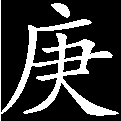
\includegraphics[width=3mm]{../Images/00004}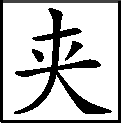
\includegraphics[width=3mm]{../Images/00012}\footnotesize \kaishu 夏日何得有桂?又桂花时节焉得又有雪?三事原系风马牛,今若强凑合,故终不相符。来此败运之事,大都如此,当局者自不解耳。}宝玉笑问道:{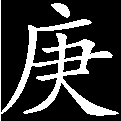
\includegraphics[width=3mm]{../Images/00004}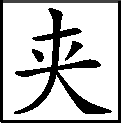
\includegraphics[width=3mm]{../Images/00012}\footnotesize \kaishu 听得``桂花''{(回)}{[}名{]}号原觉新雅,故不由一笑,余亦欲笑问。}``如何又称为`桂花夏家'?''香菱道:``他家本姓夏,非常的富贵。其馀田地不用说,单有几十顷地独种桂花,凡这长安城里城外桂花局俱是他家的,连宫里一应陈设盆景亦是他家贡奉,因此才有这个浑号。如今太爷也没了,只有老奶奶带着一个亲生的姑娘过活,也并没有哥儿兄弟,可惜他竟一门尽绝了后。''

宝玉忙道:``咱们也别管他绝后不绝后,只是这姑娘可好?你们大爷怎么就中意了?''{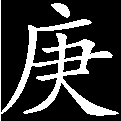
\includegraphics[width=3mm]{../Images/00004}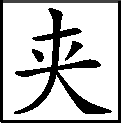
\includegraphics[width=3mm]{../Images/00012}\footnotesize \kaishu 补出阿呆素日难得中意来。}香菱笑道:``一则是天缘,二则是`情人眼里出西施'。当年又是通家来往,从小儿都一处厮混过。叙起亲是姑舅兄妹,又没嫌疑。虽离开了这几年,前儿一到他家,夏奶奶又是没儿子的,一见了你哥哥出落的这样,又是哭,又是笑,竟比见了儿子的还胜。又令他兄妹相见,谁知这姑娘出落得花朵似的了,在家里也读书写字,所以你哥哥当时就一心看准了。连当铺里老朝奉伙计们一群人蹧扰了人家三四日,他们还留多住几日,好容易苦辞才放回家。你哥哥一进门,就咕咕唧唧求我们奶奶去求亲。我们奶奶原也是见过这姑娘的,且又门当户对,也就依了。和这里姨太太、凤姑娘商议了,打发人去一说就成了。只是娶的日子太急,所以我们忙乱的很。{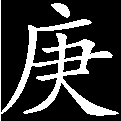
\includegraphics[width=3mm]{../Images/00004}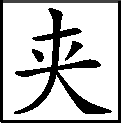
\includegraphics[width=3mm]{../Images/00012}\footnotesize \kaishu 阿呆求妇一段文字却从香菱口中补明,省却许多闲文累笔。}我也巴不得早些过来,又添一个作诗的人了。''{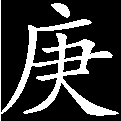
\includegraphics[width=3mm]{../Images/00004}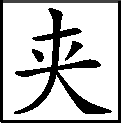
\includegraphics[width=3mm]{../Images/00012}\footnotesize \kaishu 妙极!香菱口声,断不可少。看他下``作{(死)}{[}诗{]}''语,知其心中略无忌讳疑虑等意,直是浑然天真之{[}人{]},余为一哭。}宝玉冷笑道:{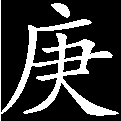
\includegraphics[width=3mm]{../Images/00004}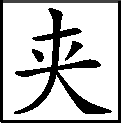
\includegraphics[width=3mm]{../Images/00012}\footnotesize \kaishu 忽曰``冷笑道'',二字便有文章。}``虽如此说,但只我倒替你耽心虑后呢。''{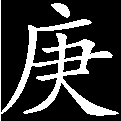
\includegraphics[width=3mm]{../Images/00004}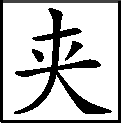
\includegraphics[width=3mm]{../Images/00012}\footnotesize \kaishu 又为香菱之谶,偏是此等事体等到。}香菱听了,不觉红了脸,正色道:``这是什么话!素日咱们都是厮抬厮敬的,今日忽然提起这些事来,是什么意思!怪不得人人都说你是个亲近不得的人。''一面说,一面转身走了。

宝玉见他这样,便怅然如有所失,呆呆的站了半天,思前想后,不觉滴下泪来,只得没精打彩,还入怡红院来。一夜不曾安稳,睡梦之中犹唤晴雯,或魇魔惊怖,种种不宁。次日便懒进饮食,身体作热。此皆近日抄检大观园、逐司棋、别迎春、悲晴雯等羞辱惊恐悲凄之所致,兼以风寒外感,故酿成一疾,卧床不起。贾母听得如此,天天亲来看视。王夫人心中自悔不合因晴雯过于逼责了他。心中虽如此,脸上却不露出。只吩咐众奶娘等好生伏侍看守,一日两次带进医生来诊脉下药。一月之后,方才渐渐的痊愈。贾母命好生保养,过百日方许动荤腥油面等物,方可出门行走。这一百日内,连院门前皆不许到,只在房中顽笑。四五十日后,就把他拘约的火星乱迸,那里忍耐得住。虽百般设法,无奈贾母王夫人执意不从,也只得罢了。因此和那些丫鬟们无所不至,恣意耍笑作戏。又听得薛蟠摆酒唱戏,热闹非常,已娶亲入门,闻得这夏家小姐十分俊俏,也略通文翰,宝玉恨不得就过去一见才好。

再过些时,又闻得迎春出了阁。宝玉思及当时姊妹们一处,耳鬓厮磨,从今一别,纵得相逢,也必不似先前那等亲密了。眼前又不能去一望,真令人凄惶迫切之至。少不得潜心忍耐,暂同这些丫鬟们厮闹释闷,幸免贾政责备逼迫读书之难。这百日内,只不曾拆毁了怡红院,和这些丫头们无法无天,凡世上所无之事,都顽耍出来。如今且不消细说。

且说香菱自那日抢白了宝玉之后,心中自为宝玉有意唐突他,``怨不得我们宝姑娘不敢亲近,可见我不如宝姑娘远矣;怨不得林姑娘时常和他角口气的痛哭,自然唐突他也是有的了。从此倒要远避他才好。''因此,以后连大观园也不轻易进来。日日忙乱着,薛蟠娶过亲,自为得了护身符,自己身上分去责任,到底比这样安宁些;二则又闻得是个有才有貌的佳人,自然是典雅和平的。因此,他心中盼过门的日子比薛蟠还急十倍。好容易盼得一日娶过了门,他便十分殷勤小心伏侍。

原来这夏家小姐今年方十七岁,生得亦颇有姿色,亦颇识得几个字。若论心中的丘壑经纬,颇步熙凤之后尘。只吃亏了一件,从小时父亲去世的早,又无同胞弟兄,寡母独守此女,娇养溺爱,不啻珍宝,凡女儿一举一动,彼母皆百依百随,因此未免娇养太过,竟酿成个盗跖的性气。爱自己尊若菩萨,窥他人秽如粪土;外具花柳之姿,内秉风雷之性。在家中时常就和丫鬟们使性弄气,轻骂重打的。今日出了阁,自为要作当家的奶奶,比不得作女儿时腼腆温柔,须要拿出这威风来,才钤压得住人;况且见薛蟠气质刚硬,举止骄奢,若不趁热灶一气炮制熟烂,将来必不能自竖旗帜矣;又见有香菱这等一个才貌俱全的爱妾在室,越发添了``宋太祖灭南唐''之意,``卧榻之侧岂容他人酣睡''之心。因他家多桂花,他小名就唤做金桂。他在家时不许人口中带出金桂二字来,凡有不留心误道一字者,他便定要苦打重罚才罢。他因想桂花二字是禁止不住的,须另换一名,因想桂花曾有广寒嫦娥之说,便将桂花改为嫦娥花,又寓自己身分如此。

薛蟠本是个怜新弃旧的人,且是有酒胆无饭力的,如今得了这样一个妻子,正在新鲜兴头上,凡事未免尽让他些。那夏金桂见了这般形景,便也试着一步紧似一步。一月之中,二人气概还都相平;至两月之后,便觉薛蟠的气概渐次低矮了下去。一日薛蟠酒后,不知要行何事,先与金桂商议,金桂执意不从。薛蟠忍不住便发了几句话,赌气自行了,这金桂便气的哭如醉人一般,茶汤不进,装起病来。请医疗治,医生又说``气血相逆,当进宽胸顺气之剂。''

薛姨妈恨的骂了薛蟠一顿,说:``如今娶了亲,眼前抱儿子了,还是这样胡闹。人家凤凰蛋似的,好容易养了一个女儿,比花朵儿还轻巧,原看的你是个人物,才给你作老婆。你不说收了心安分守己,一心一计和和气气的过日子,还是这样胡闹,噇嗓了黄汤,折磨人家。这会子花钱吃药白遭心。''一席话说的薛蟠后悔不迭,反来安慰金桂。金桂见婆婆如此说丈夫,越发得了意,便装出些张致来,总不理薛蟠。薛蟠没了主意,惟自怨而已,好容易十天半月之后,才渐渐的哄转过金桂的心来,自此便加一倍小心,不免气概又矮了半截下来。

那金桂见丈夫旗纛渐倒,婆婆良善,也就渐渐的持戈试马起来。先时不过挟制薛蟠,后来倚娇作媚,将及薛姨妈,又将至薛宝钗。宝钗久察其不轨之心,每随机应变,暗以言语弹压其志。金桂知其不可犯,每欲寻隙,又无隙可乘,只得曲意附就。一日金桂无事,因和香菱闲谈,问香菱家乡父母。香菱皆答忘记,金桂便不悦,说有意欺瞒了他。因问他``香菱''二字是谁起的名字,香菱便答:``姑娘起的。''金桂冷笑道:``人人都说姑娘通,只这一个名字就不通。''香菱忙笑道:``嗳哟,奶奶不知道,我们姑娘的学问连我们姨老爷时常还夸呢。''欲明后事,且见下回。

{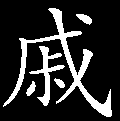
\includegraphics[width=3mm]{../Images/00005}\kaishu 总评:作诔后,黛玉飘然而至,增一番感慨,及说至迎春事,遂飘然而去。作词后,香菱飘然而至,增一番感慨,及说至薛蟠事,遂飘然而去。一点一逗,为下文引线。且二段俱以``正经事''三字作眼,而正经里更有大不正经者在,文家固无一呆字死句。}

{\kaishu 从起名上设色,别有可玩。}
